\begin{frame}[label=IF_basis]
    \frametitle{How Do We Locate Meteors?}
    \begin{columns}
        \begin{column}{0.6\textwidth}
            Through \alert{interferometry}:
            {\setlength{\leftmargini}{1em} %
            \begin{enumerate} \footnotesize
                \item<+-> Each \textcolor{blue}{\textbf{TX}} antenna sends out a unique signal
                \item<+-> Each signal takes slightly different paths
                % \begin{itemize}
                    % \item The signal whose antenna is closest to the meteor will arrive first
                    % \item The signal whose antenna is furthest to the meteor will arrive last 
                    % \item[\(\blacktriangleright\)] Each antenna is a different distance from the meteor
                    % \item[\(\blacktriangleright\)] {Each point in the sky will have a unique(ish) set of signal delays}
                    % \item E.g., for a meteor directly north of the array: the north antenna's signal will arrive before the south antenna's signal 
                % \end{itemize} 
                \item<+-> Signals bounce off the meteor trail towards \textcolor{red}{\textbf{RX}}
                \item<+-> \textcolor{red}{\textbf{RX}} measures each signal's phase
                \item<+-> Math is used to find the direction of arrival that best fits the signals' relative phases
            \end{enumerate}}
        \end{column}
        \begin{column}{0.5\textwidth}
            \centering
            \begin{tikzpicture}
                \node[anchor=south west, inner sep=0] (image) at (0,0) {%
                    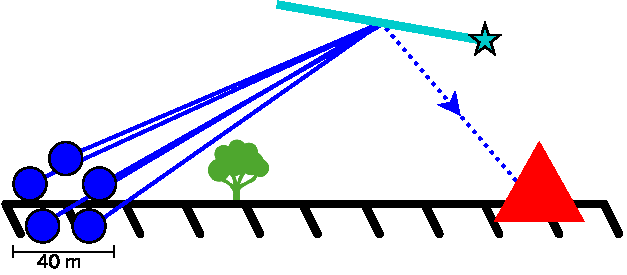
\includegraphics[width=\linewidth]{img/IF_basis.pdf}
                };
                \node<1->[circle, draw=yellow, fill=yellow!30, thick, minimum size=1mm] 
                at ([xshift=-2cm, yshift=0cm]image.center) {\scriptsize 1};
                \uncover<2->{\node[circle, draw=yellow, fill=yellow!30, thick, minimum size=1mm] 
                at ([xshift=0.8cm, yshift=0.2cm]image.north) {\scriptsize  2};}
                \uncover<3->{\node[circle, draw=yellow, fill=yellow!30, thick, minimum size=1mm] 
                at ([xshift=1.25cm, yshift=0cm]image.center) {\scriptsize  3};}
                \uncover<4->{\node[circle, draw=yellow, fill=yellow!30, thick, minimum size=1mm] 
                at ([xshift=-0.25cm, yshift=1cm]image.south east) {\scriptsize 4};}
                \uncover<5->{\node[circle, draw=yellow, fill=yellow!30, thick, minimum size=1mm] 
                (five) at ([xshift=-0.25cm, yshift=-0.5cm]image.south east) {\scriptsize 5};}
                \uncover<5->{\node[anchor = east] at ([xshift=0.1cm]five.west) { 
                    \uncovergraphics<5->[width=0.75cm]{img/calc.pdf}
                };}
        \end{tikzpicture}
        \end{column}
    \end{columns}
    \centering \uncover<6->{\hl{\textbf{Each point in the sky will have a unique* set of signal delays}}} \\ ~ \\

    \uncover<6->{\tiny *\textit{with a high SNR, good array geometry, and a well-calibrated link}}
\end{frame}